\documentclass[UTF8,a4paper,12pt]{ctexart}
\usepackage{geometry,amsmath,booktabs,graphicx,float,subcaption,hyperref}
\geometry{left=2.6cm,right=2.6cm,top=2.5cm,bottom=2.5cm}
\title{基于机器学习的心力衰竭患者随访期死亡风险预测模型构建与评估}
\author{}
\date{}
\begin{document}
\maketitle

\begin{abstract}
目的：基于心力衰竭临床记录数据，构建并比较机器学习模型对患者随访期死亡风险的预测表现。方法：纳入299名患者及12项临床特征，以DEATH\_EVENT为二分类结局，按8:2分层抽样划分训练集和测试集，比较逻辑回归、随机森林、XGBoost，并将MLP作为补充模型。结果：在60例测试集中，随机森林取得最高AUC（0.8973），Accuracy、Precision、Recall和F1分别为0.8333、0.8000、0.6316和0.7059。结论：随机森林在本实验测试集上表现相对较好，但仍需更大样本及外部验证。
\end{abstract}
\noindent\textbf{关键词：} 心力衰竭；死亡风险预测；机器学习；随机森林；ROC曲线

\section{引言（Background/Introduction）}
心力衰竭患者的临床表现和预后存在异质性，识别随访期间死亡风险较高的患者，有助于开展风险分层和个体化随访。机器学习方法能够从多维临床变量中识别潜在关系，为传统风险评估提供补充。本研究基于心衰临床记录数据，比较三种传统机器学习模型，并以多层感知机作为补充模型。

\section{资料与方法（Materials and Methods）}
\subsection{研究数据与结局定义}
数据集包含299名患者及12项临床特征。死亡96例（32.11\%），存活203例；年龄范围40--95岁，均值60.8岁。结局变量为DEATH\_EVENT（1=死亡，0=存活）。特征包括age、anaemia、creatinine\_phosphokinase、diabetes、ejection\_fraction、high\_blood\_pressure、platelets、serum\_creatinine、serum\_sodium、sex、smoking和time。

\begin{table}[H]\centering
\caption{数据集及特征概述}
\begin{tabular}{ll}\toprule
项目&描述\\\midrule
总样本量&299\\
临床特征数&12\\
死亡事件&96（32.11\%）\\
存活&203\\
年龄范围&40--95岁\\
平均年龄&60.8岁\\
训练集/测试集&239/60（8:2分层抽样）\\
训练集正类比例&32.22\%\\
测试集正类比例&31.67\%\\\bottomrule
\end{tabular}\end{table}

\subsection{数据预处理与特征分析}
数据无缺失值。采用IQR方法识别异常值，并结合临床意义保留具有合理临床解释的观测。按8:2比例分层抽样，设置stratify=y、random\_state=42，训练集239例、测试集60例。逻辑回归与MLP使用StandardScaler，且仅在训练集拟合标准化参数；随机森林和XGBoost使用原始特征。采用t检验/Welch检验结合随机森林特征重要性综合排序，前四位为time、ejection\_fraction、serum\_creatinine和age。

\begin{figure}[H]\centering
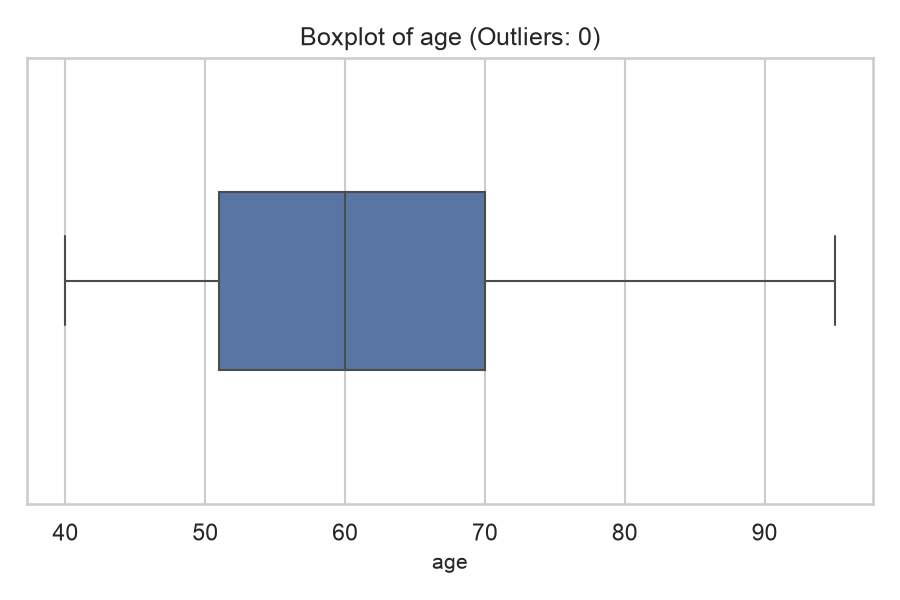
\includegraphics[width=0.82\textwidth]{box_age.png}
\caption{age}\end{figure}
\begin{figure}[H]\centering
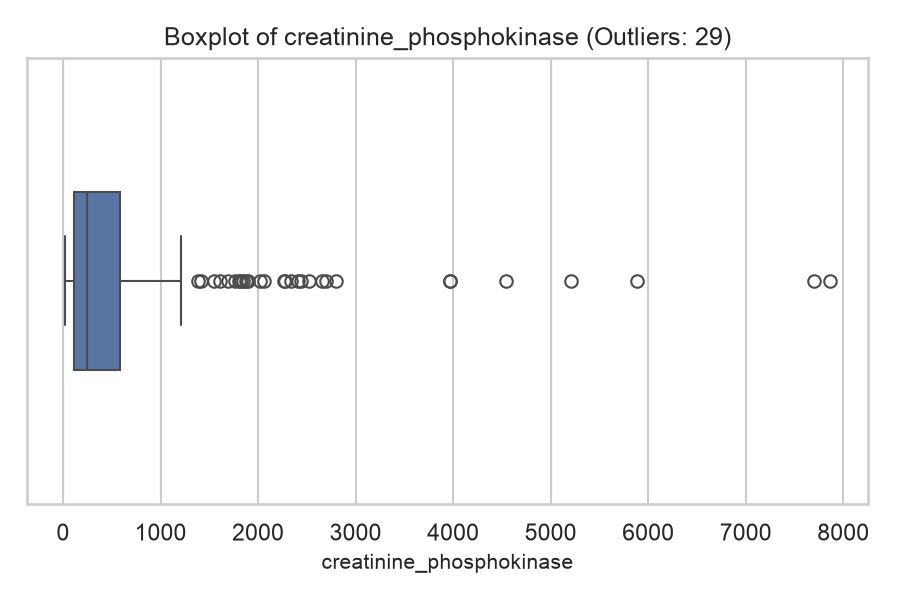
\includegraphics[width=0.82\textwidth]{box_creatinine_phosphokinase.png}
\caption{creatinine\_phosphokinase}\end{figure}
\begin{figure}[H]\centering
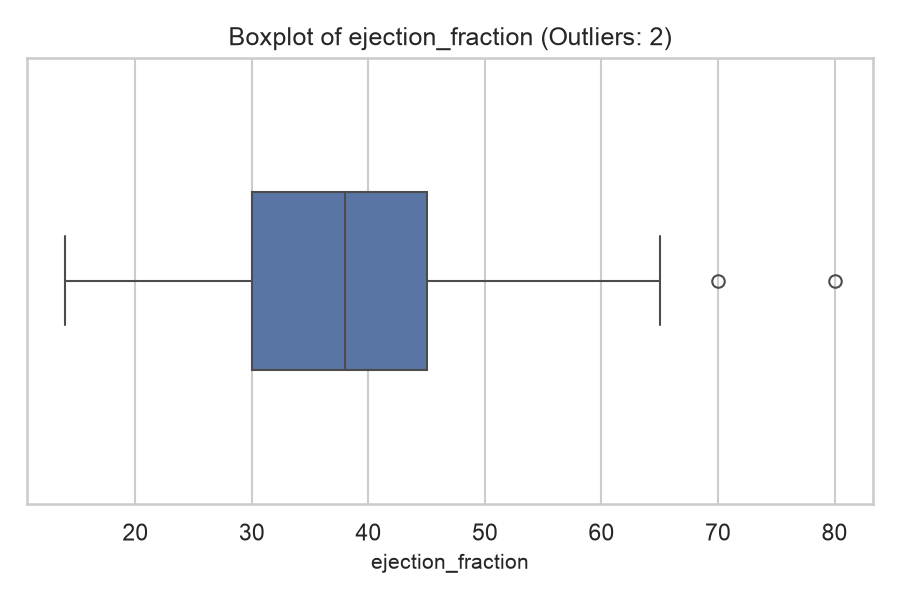
\includegraphics[width=0.82\textwidth]{box_ejection_fraction.png}
\caption{ejection\_fraction}\end{figure}
\begin{figure}[H]\centering
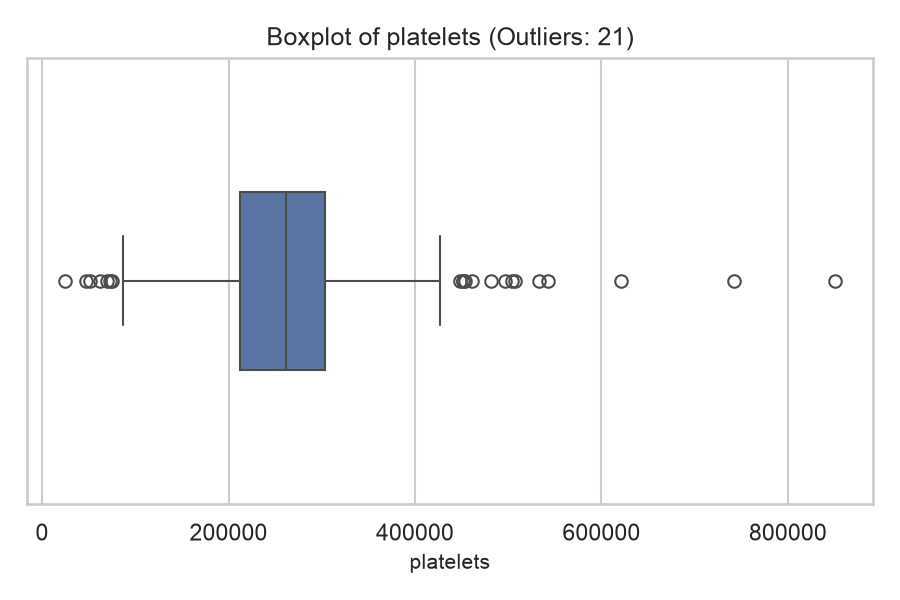
\includegraphics[width=0.82\textwidth]{box_platelets.png}
\caption{platelets}\end{figure}
\begin{figure}[H]\centering
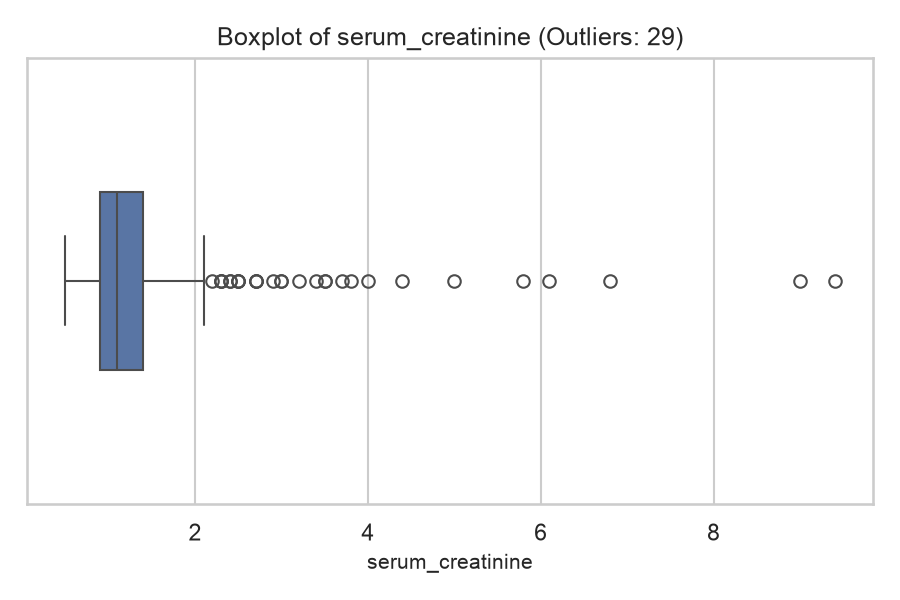
\includegraphics[width=0.82\textwidth]{box_serum_creatinine.png}
\caption{serum\_creatinine}\end{figure}
\begin{figure}[H]\centering
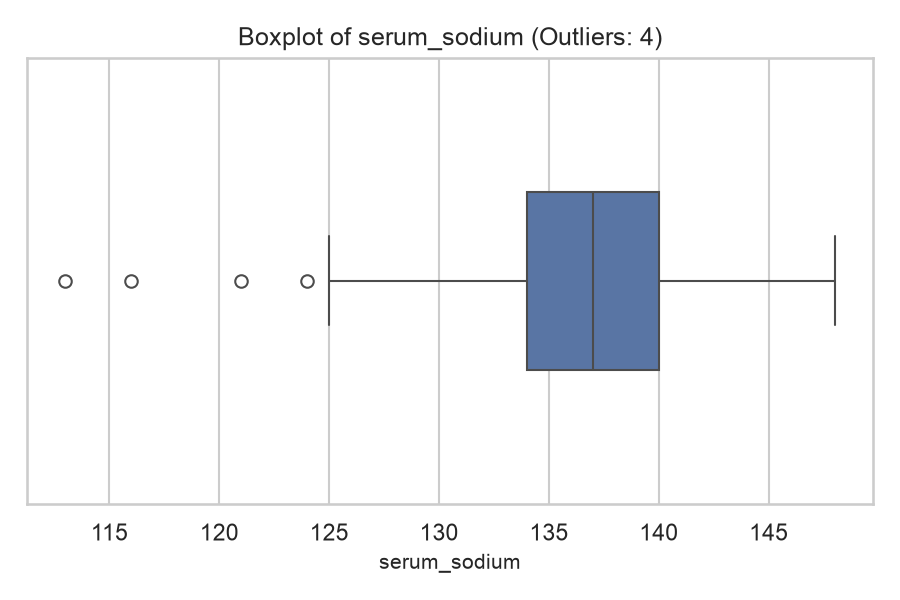
\includegraphics[width=0.82\textwidth]{box_serum_sodium.png}
\caption{serum\_sodium}\end{figure}
\begin{figure}[H]\centering
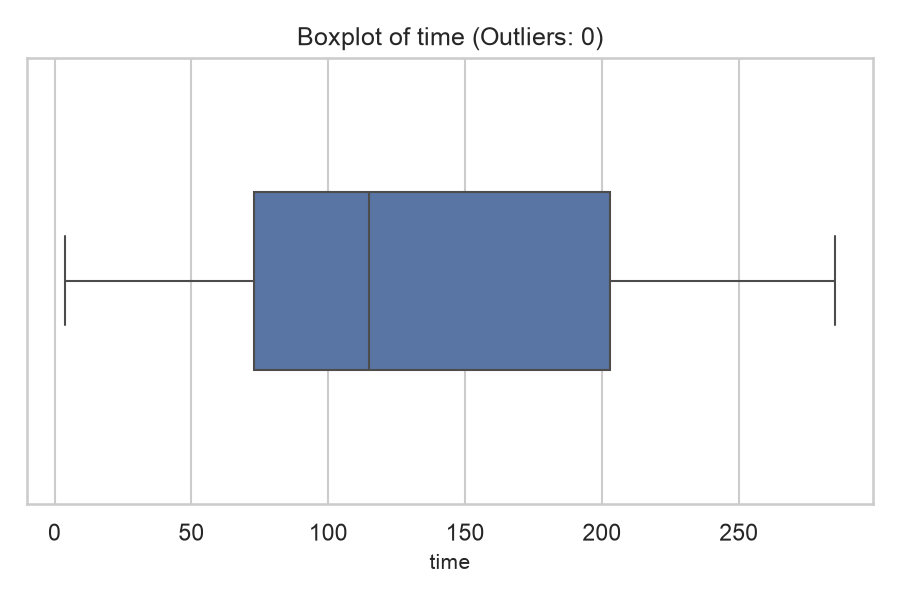
\includegraphics[width=0.82\textwidth]{box_time.png}
\caption{time}\end{figure}
\subsection{模型构建与评价}
Logistic Regression、Random Forest和XGBoost为传统机器学习主对比模型，MLP为补充模型。测试集评价指标包括Accuracy、Precision、Recall、F1-score和AUC，并绘制ROC曲线。指标定义如下：
\begin{align}
\mathrm{Accuracy}&=\frac{TP+TN}{TP+TN+FP+FN},\\
\mathrm{Precision}&=\frac{TP}{TP+FP},\qquad
\mathrm{Recall}=\frac{TP}{TP+FN},\\
F_1&=2\frac{\mathrm{Precision}\times\mathrm{Recall}}
{\mathrm{Precision}+\mathrm{Recall}}.
\end{align}

\section{结果（Results）}
\subsection{模型性能比较}
\begin{table}[H]\centering
\caption{不同模型在测试集上的性能比较}
\begin{tabular}{lccccc}\toprule
模型&Accuracy&Precision&Recall&F1-score&AUC\\\midrule
Random Forest&0.8333&0.8000&0.6316&0.7059&0.8973\\
XGBoost&0.8333&0.8462&0.5789&0.6875&0.8652\\
Logistic Regression&0.8167&0.7857&0.5789&0.6667&0.8588\\
MLP（补充）&0.7000&0.5333&0.4211&0.4706&0.7677\\\bottomrule
\end{tabular}\end{table}

\subsection{ROC曲线}
\begin{figure}[H]\centering
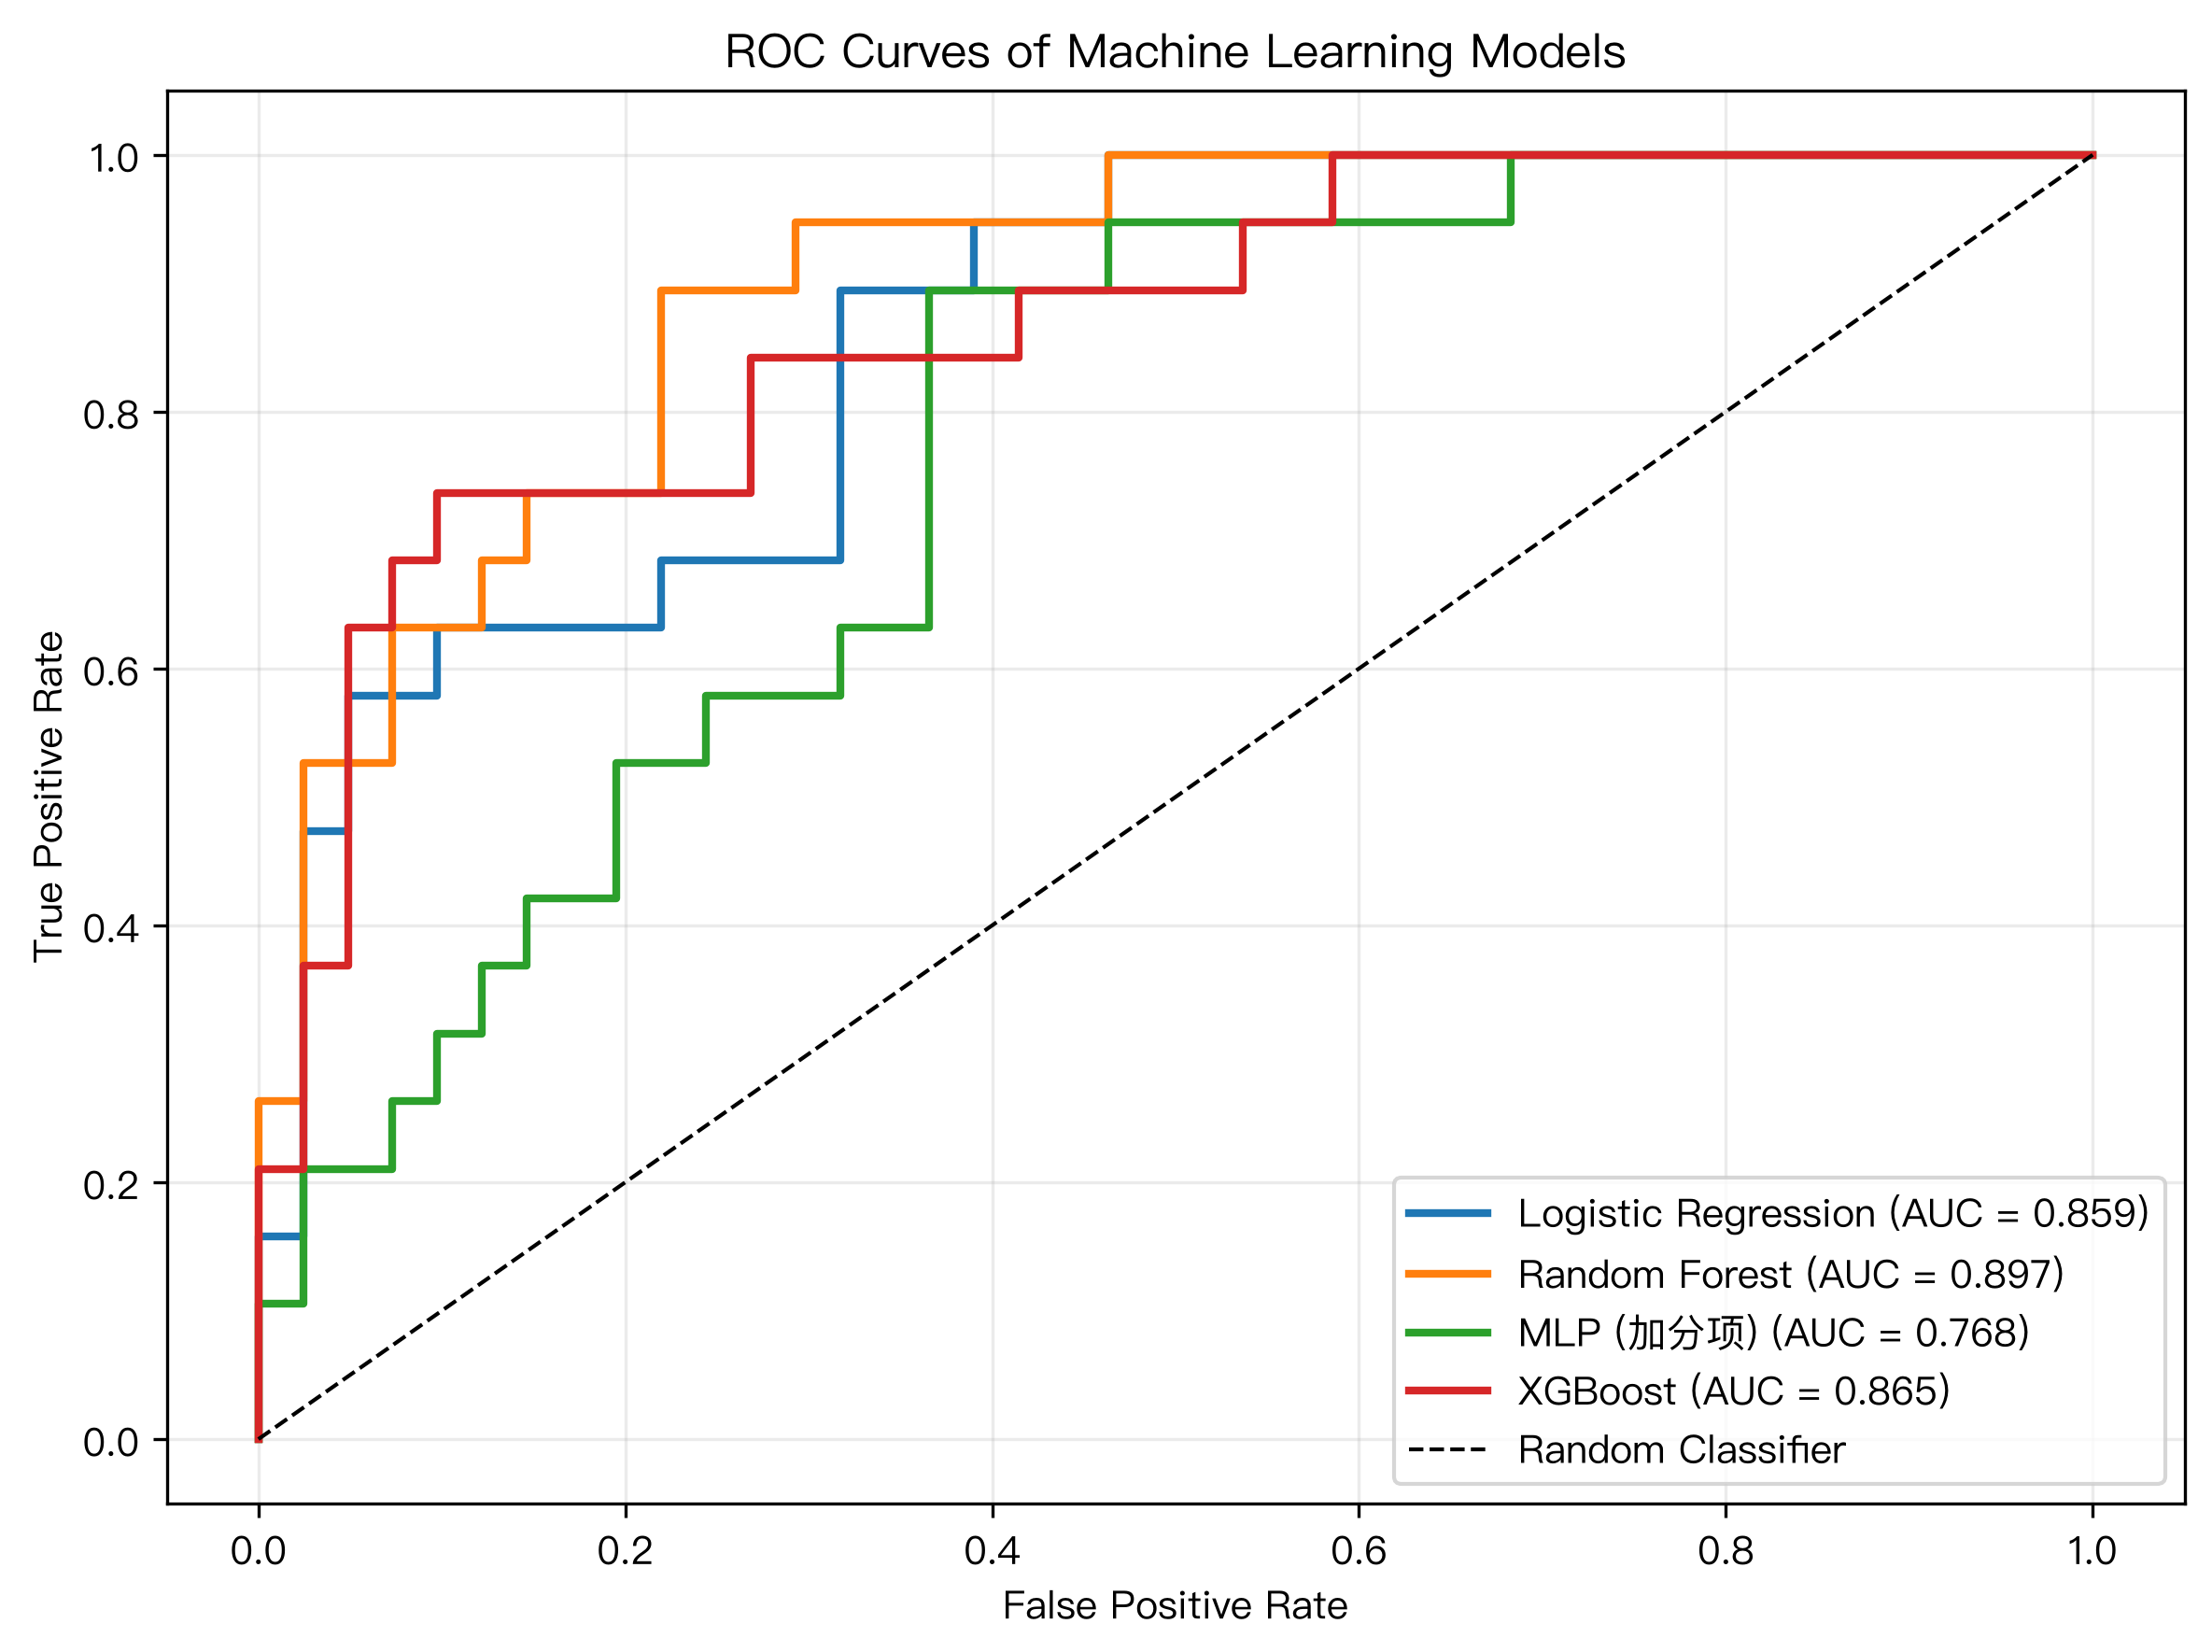
\includegraphics[width=0.88\textwidth]{三种模型_ROC曲线.png}
\caption{不同机器学习模型的ROC曲线}\end{figure}

\subsection{新患者预测示例}
患者1（78岁，贫血、糖尿病、高血压，射血分数25，血肌酐2.6，血钠131，吸烟，随访30天）的死亡概率：LR 98.01\%、RF 84.32\%、MLP 99.72\%、XGBoost 98.68\%。患者2（52岁，无贫血、糖尿病及高血压，射血分数45，血肌酐1.0，血钠139，不吸烟，随访180天）的死亡概率：LR 1.99\%、RF 2.27\%、MLP 0.00\%、XGBoost 3.38\%。上述概率仅为模型输出示例，不构成个体诊断。

\begin{figure}[H]\centering
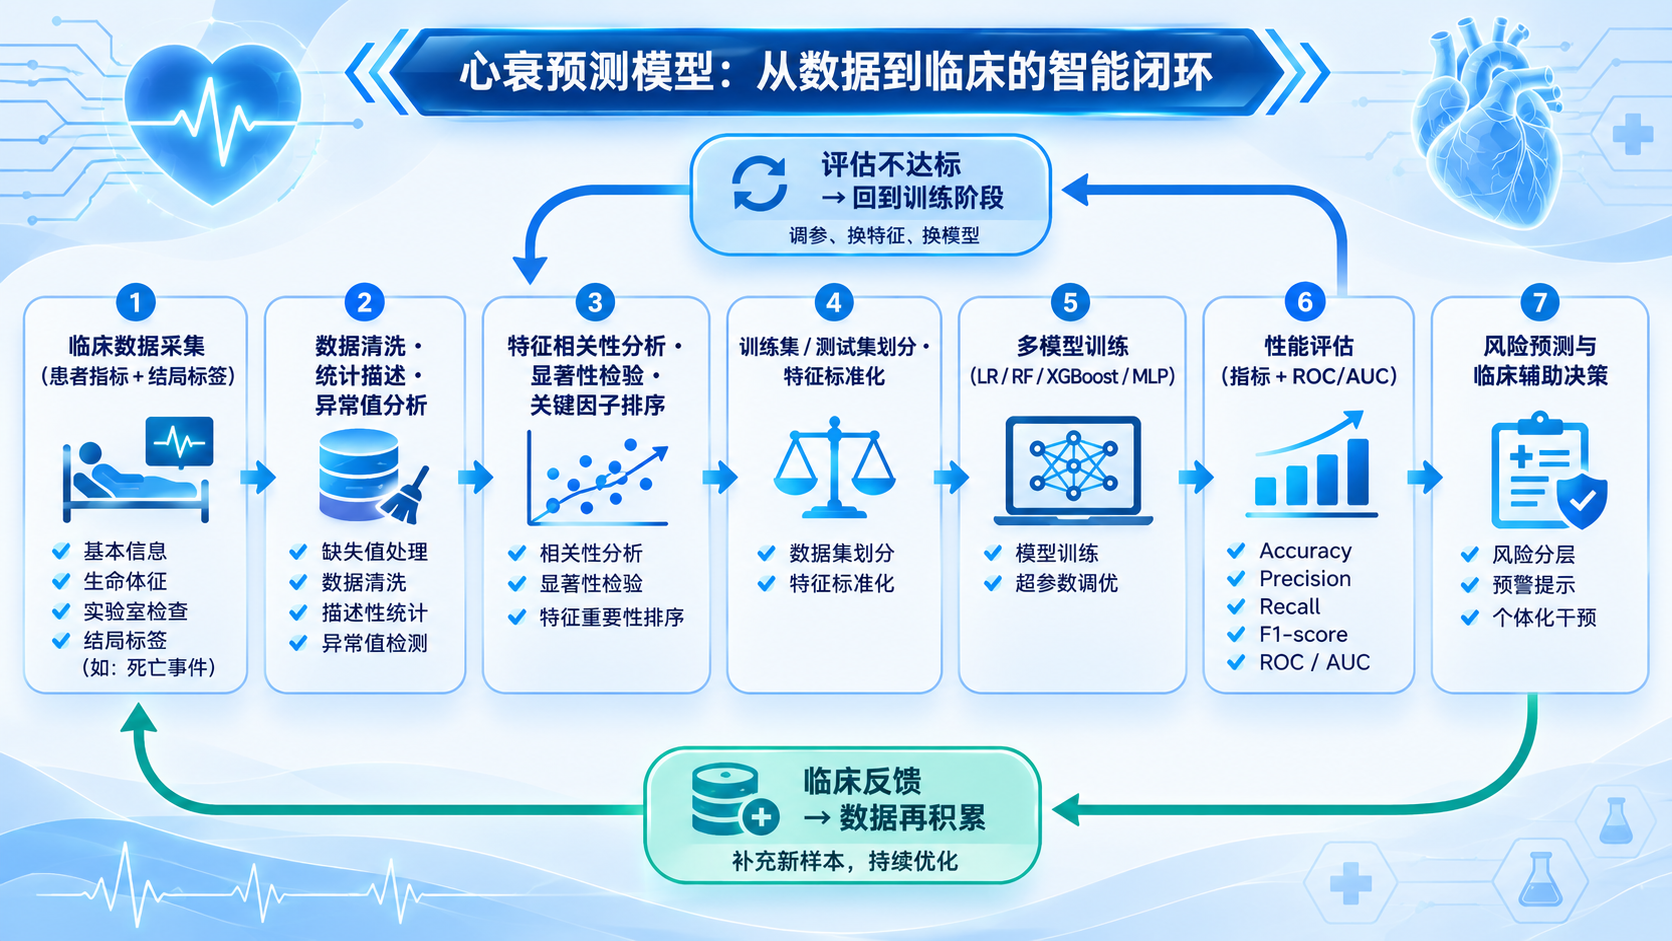
\includegraphics[width=0.92\textwidth]{心衰预测智能闭环流程图.png}
\caption{心衰死亡风险预测模型流程图）}\end{figure}

\section{讨论（Discussion）}
随机森林在测试集上取得最高AUC（0.8973），整体表现相对较好。XGBoost的Precision最高（0.8462），但Recall为0.5789。逻辑回归AUC为0.8588，与XGBoost接近。样本量仅299例时，MLP表现偏弱（AUC=0.7677），较复杂的神经网络可能难以从有限样本中稳定学习，并存在过拟合风险。各模型Recall普遍不高，提示仍可能漏报部分实际发生死亡事件的高危患者，不能仅依据Accuracy或AUC判断临床适用性。

特征综合排序前四位为time、ejection\_fraction、serum\_creatinine和age。需要注意，time属于随访时长或观察窗口，并非基线生理指标，其重要性可能与结局观察过程及数据结构有关，解读需谨慎。

本研究局限包括：样本量较小；研究数据来源及代表性有限；缺乏独立外部验证；此外，time变量的时间属性需要在实际预测时点加以审慎处理。后续应扩大样本规模，开展多中心外部验证，并评估模型在真实临床流程中的表现。

\section{结论}
机器学习模型可为心衰患者随访期死亡风险的辅助分层提供参考。本实验中随机森林取得最高AUC，但模型仍存在漏报风险，且结果受小样本和缺乏外部验证限制。未来需在更大样本和独立外部队列中进一步验证。



\begin{thebibliography}{99}

\bibitem{Adatya2026}
Adatya S, Naidu AS, Lee KK, Ambrosy AP, Axelrod AW, Dinh HH, et al.
Enhancing risk stratification for incident systolic heart failure through machine learning and natural language processing.
\textit{American Heart Journal}. 2026;292:107280.
doi:10.1016/j.ahj.2025.09.012.

\bibitem{Alba2013}
Alba AC, Agoritsas T, Jankowski M, Courvoisier D, Walter SD, Guyatt GH, et al.
Risk prediction models for mortality in ambulatory patients with heart failure: a systematic review.
\textit{Circulation: Heart Failure}. 2013;6(5):881--889.
doi:10.1161/CIRCHEARTFAILURE.112.000043.

\bibitem{Adler2020}
Adler ED, Voors AA, Klein L, Macheret F, Braun OO, Urey MA, et al.
Improving risk prediction in heart failure using machine learning.
\textit{European Journal of Heart Failure}. 2020;22(1):139--147.
doi:10.1002/ejhf.1628.

\bibitem{Lv2021}
Lv H, Yang X, Wang B, Wang S, Du X, Tan Q, et al.
Machine Learning-Driven Models to Predict Prognostic Outcomes in Patients Hospitalized With Heart Failure Using Electronic Health Records: Retrospective Study.
\textit{Journal of Medical Internet Research}. 2021;23(4):e24996.
doi:10.2196/24996.

\bibitem{Negassa2021}
Negassa A, Ahmed S, Zolty R, Patel SR.
Prediction Model Using Machine Learning for Mortality in Patients with Heart Failure.
\textit{The American Journal of Cardiology}. 2021;153:86--93.
doi:10.1016/j.amjcard.2021.05.044.

\bibitem{Konig2021}
König S, Pellissier V, Hohenstein S, Bernal A, Ueberham L,
Meier-Hellmann A, et al.
Machine learning algorithms for claims data-based prediction of in-hospital mortality in patients with heart failure.
\textit{ESC Heart Failure}. 2021;8(4):3026--3036.
doi:10.1002/ehf2.13398.

\bibitem{Xu2025}
Xu Z, Hu Y, Shao X, Shi T, Yang J, Wan Q, et al.
The efficacy of machine learning models for predicting the prognosis of heart failure: A systematic review and Meta-Analysis.
\textit{Cardiology}. 2025;150:79--97.
doi:10.1159/000538639.

\end{thebibliography}


\end{document}
